\documentclass{article}
\usepackage{amsmath}
\usepackage{amsfonts}
\usepackage{graphicx}
\DeclareMathOperator{\deriv}{d}
\DeclareMathOperator{\diag}{diag}
\begin{document}
\section{2.14}
We will show that $x_k=1+(0.5)^{2^k}$ converges $Q$-quadratically to 1. So, by definition, we need
to find a constant $M>0$ such that
\begin{align*}
\frac{|x_{k+1}-1|}{|x_k-1|^2}\leq M
\end{align*} 
for all $k$ sufficiently large. Because of the equalities
\begin{align*}
\frac{|x_{k+1}-1|}{|x_k-1|^2}=\frac{(0.5)^{2^{k+1}}}{(0.5)^{2^{k+1}}}=1
\end{align*}
that holds for all $k$, we see that the claim follows with $M=1$.  \par
\section{2.15}
We will show that $x_k=\frac{1}{k!}$ converges $Q$-superlinearly to 0 but not $Q$-quadratically.
In order to prove the first claim, we need to show  that
\begin{align*}
\lim_{k\rightarrow \infty}\frac{|x_{k+1}|}{|x_k|}=0
\end{align*}
holds. This follows easily after simplfying the expression.
\begin{align*}
\frac{\frac{1}{(k+1)!}}{\frac{1}{k!}}=\frac{k!}{(k+1)!}=\frac{1}{k+1}\xrightarrow{k \rightarrow \infty} 0
\end{align*}
To show the latter claim, note that 
\begin{align*}
\frac{|x_{k+1}|}{|x_k|^2}=\frac{\frac{1}{(k+1)!}}{\frac{1}{k!\cdot k!}}\frac{k!}{k+1}\xrightarrow{k\rightarrow \infty} \infty
\end{align*}
which implies that there is no constant $M$ fulfilling the definition of $Q$-quadratic convergence.\section{2.16}
We will show that the sequence
\begin{align*}
x_k=\begin{cases}\left(\frac{1}{4}\right)^{2^k}, & k \textrm{ even} \\
                  \frac{x_{k-1}}{k}, & k \textrm{ odd} \end{cases}
\end{align*}
converges both $Q$-superlinearly and $R$-quadratically to zero but not $Q$-quadratically.
By
\begin{align*}
\frac{|x_{k+1}|}{|x_{k}|}=\begin{cases}\frac{x_k}{kx_k}  \\
                                      \frac{\left(1/4\right)^{2^{k+1}}k}{(1/4)^{2^{k-1}}} \end{cases}=\begin{cases} \frac{1}{k}, &  k \textrm{ even} \\
              k(1/4)^{3\cdot 2^{k-1}},  &k  \textrm{ odd} \end{cases}
\end{align*}
As both of these two sequences covnerge to zero, the claim follows. \par
To show that the sequence converges $R$-quadratically, we consider the sequence
$v_k=(1/4)^{2^{k-1}}$. Since $(1/4)^{2^k}\leq v_k $ and $(1/4)^{2^{k-1}}/k\leq v_k$, we get
$x_k\leq v_k$. Also, $v_k$ converges $Q$-quadratically, where the proof is essentially the same
as the argument given in exercise 2.14. Hence, $x_k$ converges $R$-quadratically.\par
Lastly, we will show that $x_k$ does not converge $Q$-quadratically. For $k$ even, we see that
\begin{align*}
\frac{|x_{k+1}|}{|x_k|^2}=\frac{(1/4)^{2^k}}{(k+1)\cdot\left( (1/4)^{2^k} \right)^2}
=\frac{1}{(k+1)(1/4)^{2^k}},
\end{align*}
which converges to infinity and is therefore unbounded. This implies that the sequence does not converge $Q$-quadratically.
\section{Pictures Exercise 1}
The following pictures show the convergence properties.
The first picture displays the $q=1$-quotient of $1+\left(\frac{1}{2}\right)^{2^k}$.
\begin{figure}[h!]
  \centering
  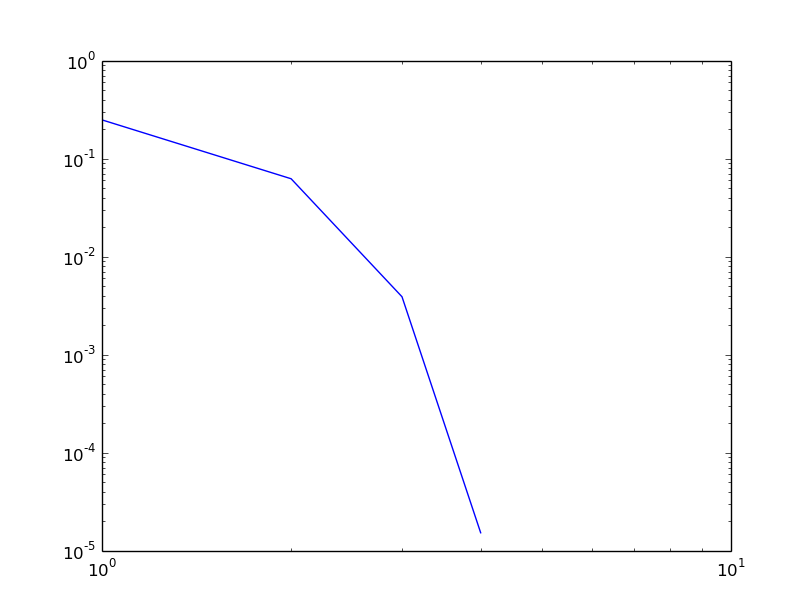
\includegraphics[scale=0.5]{f_1.png}
\end{figure}
The second picture displays the $q=1$-quotient of $\frac{1}{k!}$
\begin{figure}[h!]
  \centering
  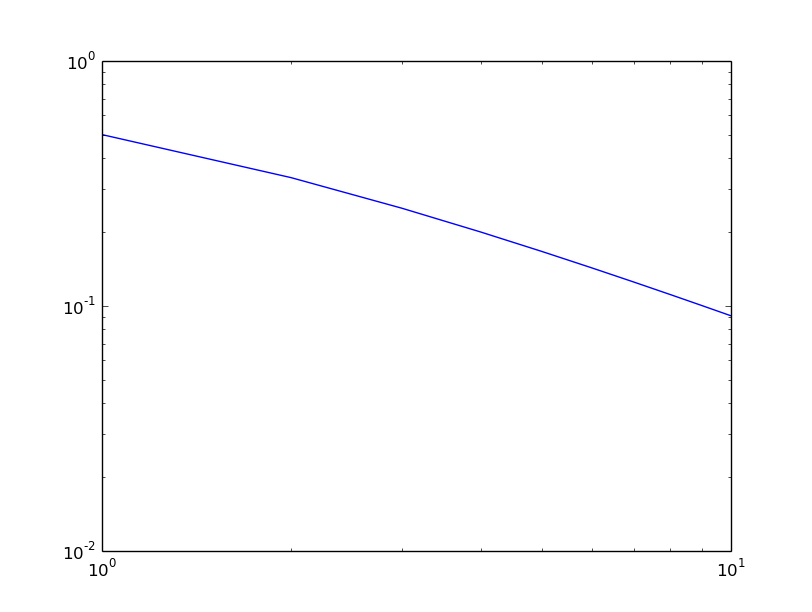
\includegraphics[scale=0.5]{g_1.png}
\end{figure}
The next two pictures show the quotient for $q=1$ and $q=2$ for the sequence from exercise 2.16.
\begin{figure}[h!]
  \centering
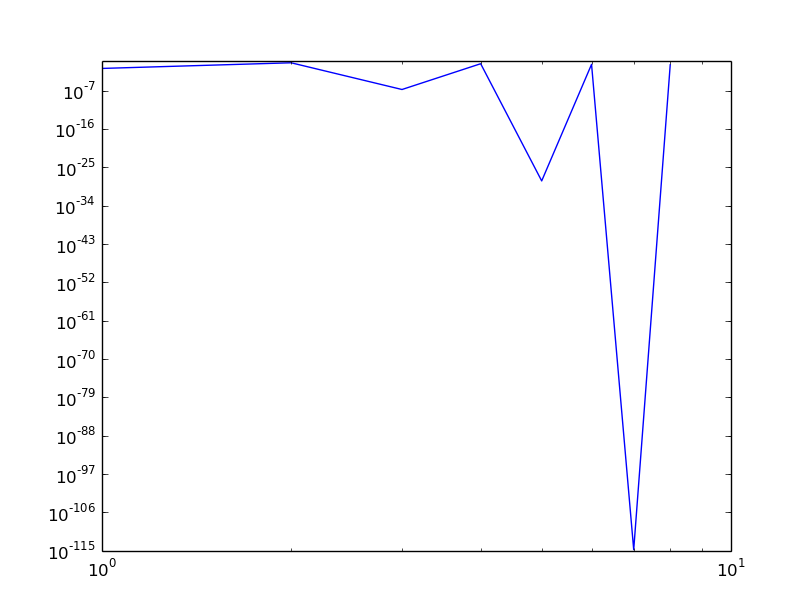
\includegraphics[scale=0.3]{h_1.png}
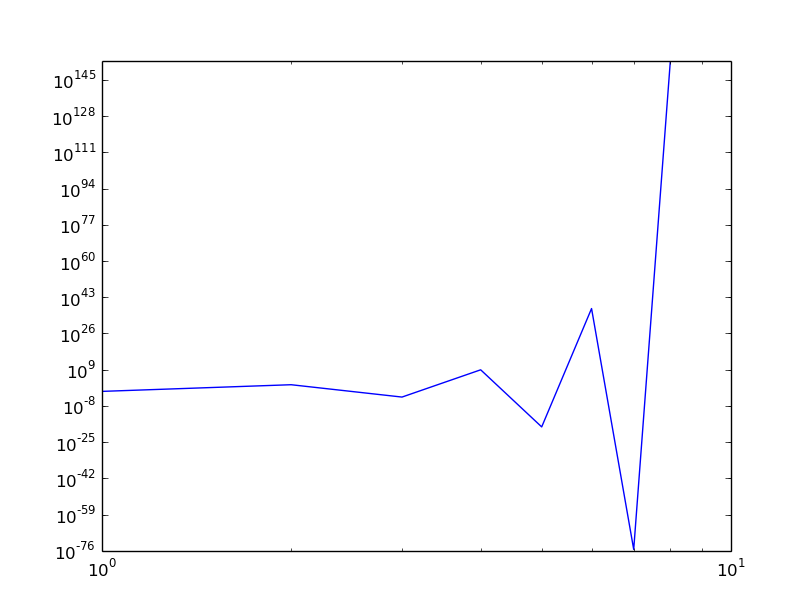
\includegraphics[scale=0.5]{h_2.png}  
\end{figure}

The last picture displays the $q=1$ quotient for $\frac{1}{k}$ which converges $q$-linearly but
not superlinearly.
\begin{figure}[h!]
  \centering
  
\end{figure}
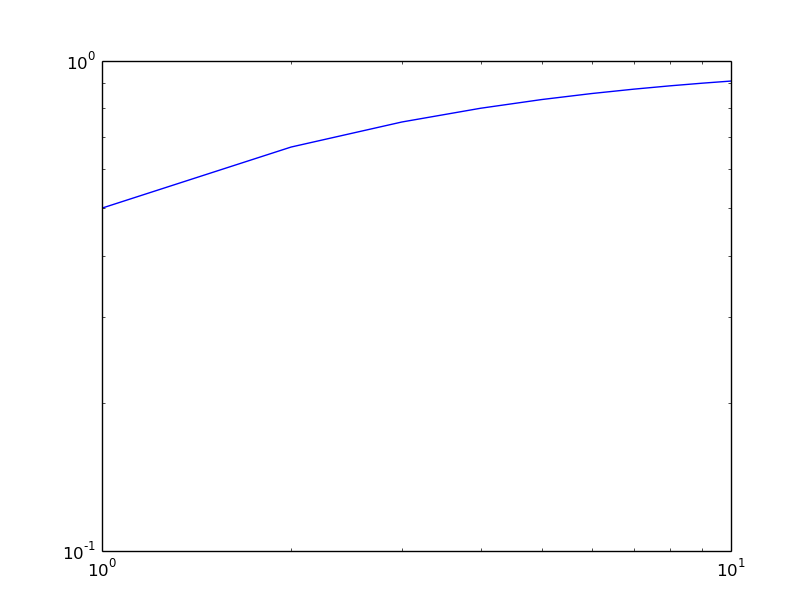
\includegraphics[scale=0.5]{r_1.png}
\section{Exercise 2}
\subsection{2.1}
We will discretize the optimization problem
\begin{align*}
  \min_{x}\int_{0}^{1} \left[\left(\frac{\deriv x_1(t)}{\deriv t}\right)^{2}+ \left(\frac{\deriv x_2(t)}{\deriv t}\right)^{2} \right]\rho(x(t)) \deriv t
\end{align*}
,subject to the condtion $x(0)=a$ and $x(1)=b$,
by discretizing $x$ on $n$ points using finite differences and the midpoint rule.
Let $t_i=\frac{i}{n}$ for $0\leq i \leq n$. 
\begin{align*}
  &\int_{0}^{1} \left[\left(\frac{\deriv x_1(t)}{\deriv t}\right)^{2}+ \left(\frac{\deriv x_2(t)}{\deriv t}\right)^{2} \right]\rho\left(x\left(t\right)\right) \deriv t\\
=&\sum_{i=o}^{n-1}\int_{t_i}^{t_{i+1}} \left[\left(\frac{\deriv x_1(t)}{\deriv t}\right)^{2}+ \left(\frac{\deriv x_2(t)}{\deriv t}\right)^{2} \right]\rho\left(x\left(t\right)\right) \deriv t\\
\approx&\sum_{i=0}^{n-1} \Delta x  \left[\left(\frac{\deriv x_1(\frac{t_i+t_{i+1}}{2})}{\deriv t}\right)^{2}+ \left(\frac{\deriv x_2(\frac{t_i+t_{i+1}}{2})}{\deriv t}\right)^{2} \right]\rho\left(x\left(\frac{t_{i}+t_{i+1}}{2}\right)\right) \deriv t\\
\approx & \sum_{i=0}^{n-1}\Delta x \left[\left(\frac{x_{1,i+1}-x_{1,i}}{\Delta x}\right)^2+
\left(\frac{x_{2,i+1}-x_{2,i}}{\Delta x}\right)^2 \right]\frac{\rho(x_{i+1})+\rho(x_i)}{2}\\
= &  \sum_{i=0}^{n-1}\frac{1}{2\Delta x}\left[\left(x_{1,i+1}-x_{1,i}\right)^2+
\left(x_{2,i+1}-x_{2,i}\right)^2 \right]\left(\rho(x_{i+1})+\rho(x_i)\right)\\
\end{align*}
We will rewrite this now using  matrix notation to facilitate differentiation.
For this, we will set
\begin{align*}
  x&=(x_{1,1},x_{1,2},\dotsc,x_{1,n-1},x_{2,1},\dotsc,x_{2,n-1})^{T} &\in \mathbb{R}^{2(n-1)} \\
  v&=(-a_{1},0,\dotsc,0,b_{1},-a_{2},0,\dotsc,0,b_{2})^{T} &\in \mathbb{R}^{2n} \\
 \rho(x)&=(\rho(x_1),\dotsc,\rho(x_{n-1}))^{T}  &\in \mathbb{R}^{n-1} \\
 w&=(\rho(a),0,\dotsc,0,\rho(b),\rho(a),\dotsc,0,\rho(b))^{T}  &\in \mathbb{R}^{2n}  \\
A'&=\begin{pmatrix}
 1& & & \\
-1&1& & \\
  &\ddots &\ddots & \\
  & &-1 &0  
\end{pmatrix}& \in \mathbb{R}^{n\times(n-1)} \\
A&=\begin{pmatrix}
A' & 0 \\
0 & A' \\
\end{pmatrix} & \in \mathbb{R}^{(2n)\times(2(n-1))} \\
M'&=\begin{pmatrix}
 1& & & \\
1&1& & \\
  &\ddots &\ddots & \\
  & &1 &0  
\end{pmatrix}& \in \mathbb{R}^{n\times(n-1)} \\
M&=
\begin{pmatrix}
M' \\
M' \\
\end{pmatrix} & \in \mathbb{R}^{(2n)\times(n-1)} 
\end{align*}
which will allow us to rewrite our discretization and define our objective function.
\begin{align*}
f:&\mathbb{R}^{2(n-1)}\rightarrow \mathbb{R} \\
x\mapsto& \frac{1}{2\Delta x} \left((Ax+v)\odot (Ax+v)\right)^{T}\left(M\rho(x)+w)\right)
\end{align*}
By use of the differentiation rules discussed in class, we get that
\begin{align*}
  \nabla f (x)=\frac{1}{2*\Delta x}\left[\nabla\rho(x)M^T(Ax+v)\odot(Ax+v)+2A^T\diag(Ax+v)(M\rho(x)+w)\right]
\end{align*}
up to transpose ;-).
\section{Pictures Exercise 2}
The following pictures show my favorite examples and one of them shows the first
20 iterations because I thought that that looks cool.
\begin{figure}[h]
  \centering
  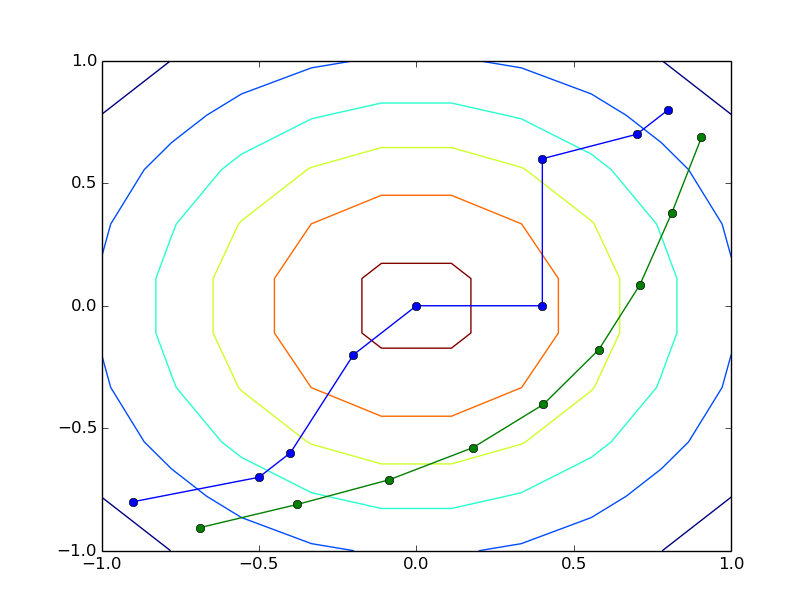
\includegraphics[scale=0.5]{ex2.png}
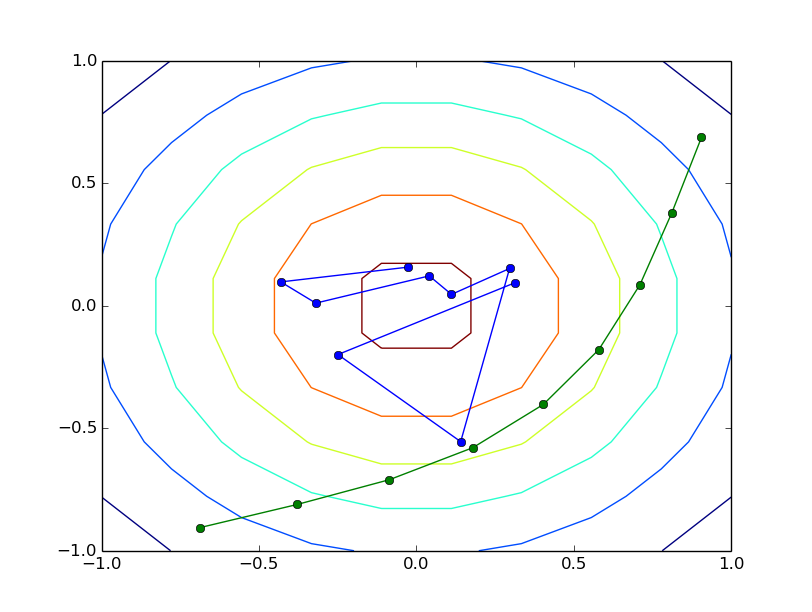
\includegraphics[scale=0.5]{ex22.png}
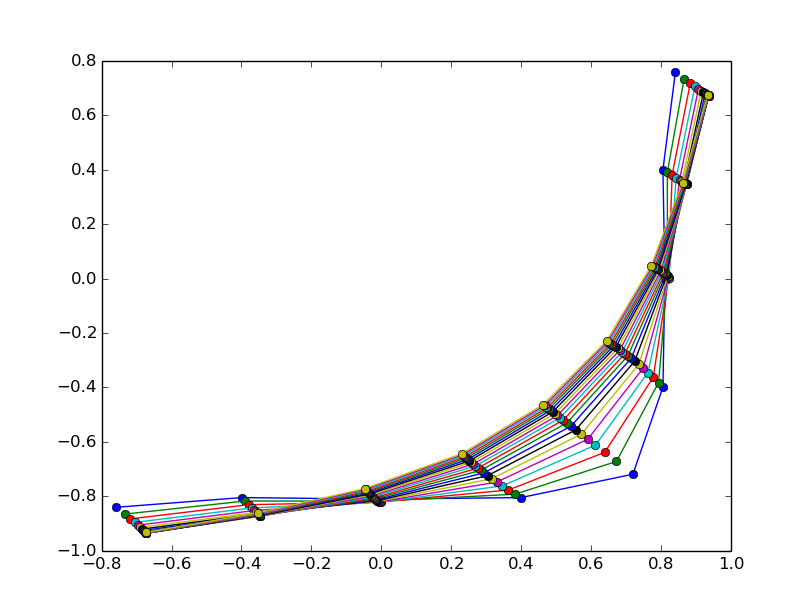
\includegraphics[scale=0.5]{ex2m.png}
\end{figure}
\end{document}